\chapter{Specyfikacja zewnętrzna}
\label{ch:04}

\section{Wymagania sprzętowe i programowe}

Program wykorzystuje potok programowalny bilbioteki OpenGL oraz jednostki cieniujące napisane w~języku GLSL w wersji 3.30, oznacza to, że~system użytkownika musi posiadać kartę graficzną wspierającą OpenGL conajmniej w~wersji 3.3.
Dodatkowo program wykorzystuje następujące biblioteki, których kod źródłowy znajduje się wewnątrz projetu:
\begin{itemize}
\item GLAD
\item GLFW
\item GLM
\item Dear ImGui
\end{itemize}

Projekt został skompilowany i~przetestowany wykorzystując kompilator g++
w~wersji 12.2.0 na~systemie Linux. Kompilacja progamu odbywa się przy pomocy narzędzia CMake.

\section{Sposób instalacji}
\subsection{System Linux}
Przykład kompilacji programu został wykonany przy wykorzystaniu systememu Ubuntu 22.04. Pierwszym krokiem jest instalacja narzędzi takich jak program cmake, kompilator języka C i C++, itp. oraz instalacja wymaganych bibliotek.
Do tego celu wykorzystane są następujące polecenia
\lstset{basicstyle=\ttfamily, language=bash}
\begin{lstlisting}[language=bash]
  sudo apt install cmake
  sudo apt install build-essential
  sudo apt install xorg-dev
  sudo apt install git
\end{lstlisting}

Następnym krokiem jest pobranie repozytorium git projektu. Istotnym jest by pobrać repozytorium rekurencyjnie, gdyż dołączone biblioteki zostały dodane do repozytorium jako submoduły. Można tego dokonać poleceniem
\begin{lstlisting}[language=bash]
  git clone https://github.com/Rei-sen/raymarch-terrain --recursive
\end{lstlisting}
Alternatywnie, jeżeli repozytorium nie zostało pobrane rekurencyjnie można zastosować polecenia
\begin{lstlisting}[language=bash]
  git submodule init
\end{lstlisting}
a następnie
\begin{lstlisting}[language=bash]
  git submodule update
\end{lstlisting}
Ostatnim krokiem jest wygenerowanie plików reguł Makefile a następnie
kompilacja projektu. Generacji plików reguł Makefile można dokonać wywołując następujące polecenie w głównym katalogu projektu
\begin{lstlisting}[language=bash]
  cmake -B build -S .
\end{lstlisting}
W celu kompilacji należy wykorzystać poniższe polecenie
\begin{lstlisting}[language=bash]
  cmake --build build
\end{lstlisting}
Końcowy plik wykonywalny o nazwie raymarch-terrain znajduje się w katalogu build.
\subsection{System Windows}

\subsection{Sposób obsługi}


Jeśli „Specyfikacja zewnętrzna”:
\begin{itemize}
\item  wymagania sprzętowe i programowe
\item  sposób instalacji
\item  sposób aktywacji
\item  kategorie użytkowników
\item  sposób obsługi
\item  administracja systemem
\item  kwestie bezpieczeństwa
\item  przykład działania
\item  scenariusze korzystania z systemu (ilustrowane zrzutami z ekranu lub generowanymi dokumentami)
\end{itemize}

%%%%%%%%%%%%%%%%%%%%%
%% RYSUNEK Z PLIKU
%
%\begin{figure}
%\centering
%
\includegraphics[width=0.5\textwidth]{./graf/politechnika_sl_logo_bw_pion_pl.pdf}
%\caption{Podpis rysunku zawsze pod rysunkiem.}
%\label{fig:etykieta-rysunku}
%\end{figure}
%Rys. \ref{fig:etykieta-rysunku} przestawia …
%%%%%%%%%%%%%%%%%%%%%
%
%%%%%%%%%%%%%%%%%%%%%
%% WIELE RYSUNKÓW
%
%\begin{figure}
%\centering
%\begin{subfigure}{0.4\textwidth}
%    
\includegraphics[width=\textwidth]{./graf/politechnika_sl_logo_bw_pion_pl.pdf}
%    \caption{Lewy górny rysunek.}
%    \label{fig:lewy-gorny}
%\end{subfigure}
%\hfill
%\begin{subfigure}{0.4\textwidth}
%    
\includegraphics[width=\textwidth]{./graf/politechnika_sl_logo_bw_pion_pl.pdf}
%    \caption{Prawy górny rysunek.}
%    \label{fig:prawy-gorny}
%\end{subfigure}
%
%\begin{subfigure}{0.4\textwidth}
%    
\includegraphics[width=\textwidth]{./graf/politechnika_sl_logo_bw_pion_pl.pdf}
%    \caption{Lewy dolny rysunek.}
%    \label{fig:lewy-dolny}
%\end{subfigure}
%\hfill
%\begin{subfigure}{0.4\textwidth}
%    
\includegraphics[width=\textwidth]{./graf/politechnika_sl_logo_bw_pion_pl.pdf}
%    \caption{Prawy dolny rysunek.}
%    \label{fig:prawy-dolny}
%\end{subfigure}
%
%\caption{Wspólny podpis kilku rysunków.}
%\label{fig:wiele-rysunkow}
%\end{figure}
%Rys. \ref{fig:wiele-rysunkow} przestawia wiele ważnych informacji, np. rys. \ref{fig:prawy-gorny} jest na prawo u góry.
%%%%%%%%%%%%%%%%%%%%%


 
\begin{figure}
\centering
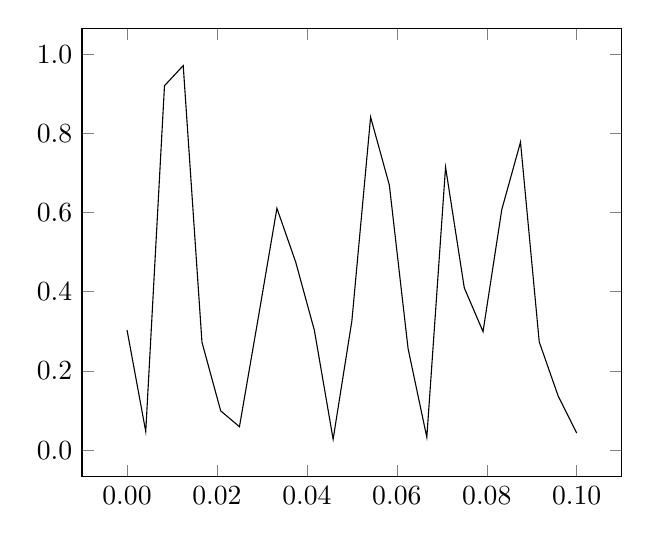
\begin{tikzpicture}
\begin{axis}[
    y tick label style={
        /pgf/number format/.cd,
            fixed,   % po zakomentowaniu os rzednych jest indeksowana wykladniczo
            fixed zerofill, % 1.0 zamiast 1
            precision=1,
        /tikz/.cd
    },
    x tick label style={
        /pgf/number format/.cd,
            fixed,
            fixed zerofill,
            precision=2,
        /tikz/.cd
    }
]
\addplot [domain=0.0:0.1] {rnd};
\end{axis} 
\end{tikzpicture}
\caption{Podpis rysunku po rysunkiem.}
\label{fig:2}
\end{figure}

